\documentclass[14pt,a4paper]{extarticle}



\usepackage[utf8]{inputenc}
\usepackage[T2A]{fontenc}
\usepackage{amssymb,amsmath,mathrsfs,amsthm}
\usepackage[russian]{babel}
\usepackage{graphicx}
\usepackage[footnotesize]{caption2}
\usepackage{indentfirst}
\usepackage{multicol}
\usepackage{listings}
\usepackage{float}
\usepackage{url}

\usepackage{enumitem}

%\usepackage[ruled,section]{algorithm}
%\usepackage[noend]{algorithmic}
%\usepackage[all]{xy}
\usepackage{booktabs}
\usepackage{graphicx}
\usepackage[table,xcdraw]{xcolor}
\usepackage{tcolorbox}

%Библиотека для блок-схем
\usepackage{tikz}
\usetikzlibrary{shapes,arrows}

% Параметры страницы
\textheight=24cm
\textwidth=16cm
\oddsidemargin=5mm
\evensidemargin=-5mm
\marginparwidth=36pt
\topmargin=-1cm
\footnotesep=3ex
%\flushbottom
\raggedbottom
\tolerance 3000
% подавить эффект "висячих стpок"
\clubpenalty=10000
\widowpenalty=10000
%\renewcommand{\baselinestretch}{1.1}
\renewcommand{\baselinestretch}{1.5} %для печати с большим интервалом

\newcommand{\angstrom}{\mbox{\normalfont\AA}}

\newtheorem{definition}{Определение} % задаём выводимое слово (для определений)
\newtheorem{example}{Замечание} % задаём выводимое слово (для определений)
\newtheorem{theorem}{Теорема} % задаём выводимое слово (для определений)
\newtheorem{construction}{Конструкция} % задаём выводимое слово (для определений)

\DeclareMathOperator*{\sgn}{sgn}
\DeclareMathOperator*{\var}{var}   
\DeclareMathOperator*{\cov}{cov}
\DeclareMathOperator*{\law}{Law}

\newcommand{\1}{\mathbbm{1}} 
\newcommand{\R}{\mathbb{R}}
\newcommand{\N}{\mathbb{N}}
\newcommand{\Z}{\mathbb{Z}}
\renewcommand{\P}{\mathbb{P}}
\newcommand{\E}{\mathbb{E}}

\newcommand{\independent}{\perp\!\!\!\!\perp}


\newcommand\cA{{\cal A}}
\newcommand\cE{{\cal E}}
\newcommand\cC{{\cal C}}
\newcommand\cF{{\cal F}}
\newcommand\cG{{\cal G}}
\newcommand\cK{{\cal K}}
\newcommand\cL{{\cal L}}
\newcommand\cB{{\cal B}}
\newcommand\cN{{\cal N}}
\newcommand\cM{{\cal M}}
\newcommand\cX{{\cal X}}
\newcommand\cD{{\cal D}}
\newcommand\cR{{\cal R}}
\newcommand\cP{{\cal P}}
\newcommand\cQ{{\cal Q}}
\newcommand\cS{{\cal S}}
\newcommand\cT{{\cal T}}
\newcommand\cV{{\cal V}}
\newcommand\cZ{{\cal Z}}

\newcommand{\textProposition}    {Предложение}

\begin{document}

\begin{center}

{Всеволод Заостровский, 409 группа}\\
{\bfseries Отчёт по задаче "Приближение с помощью построения ряда Фурье".\\}
\vspace{1cm}

\end{center}

\section{Постановка задачи.}
Для функции $u(x) \in C^{\infty}[0, 1]$, удовлетворяющей краевым условиям:
\begin{align*}
    & u(0) = u(1) = 0,
\end{align*}
необходимо выписать тригонометрический ряд Фурье и сформулировать теорему сходимости. Затем, на сетке:

\begin{align*}
    & x_0 = \frac{-h}{2}, \\
    & x_N = 1, \\
    & h = \frac{1}{N - 0.5},
\end{align*}     

выписать дискретный тригонометрический ряд Фурье. 
Найти дискретное скалярное произведение, сохраняющее ортогональность базисных функций. 
Нормировать базисные функции. 
\\
И, наконец, для некоторой тестовой функции из указанного класса численно найти порядок скодимости её дискретного ряда Фурье.

\section{Тригонометрический ряд Фурье.}
Из краевых условий видно, что функцию $u(x) \in C^{\infty}[0, 1]$ можно разложить в ряд Фурье, 
взяв синусы в качестве базисных функций:
\begin{equation*}
    u(x) = \sum_{m = 1}^{\infty} c_m \sin {\pi m x}.
\end{equation*}

Перейдём к рассмотрению конечного числа узлов. Выпишем условия на сетку:
\begin{align*}
    & u_k := u(x_k), \; h = \frac{1}{N - 0.5}, \; x_k := \frac{-h}{2} + k h \\
    & u(x_k) = \sum_{m=1}^{N - 1} c_m^N \sin{\pi m x_k}, \\
    & \phi_k^m := \sin{\pi m (\frac{-h}{2} + k h)} \\
    & \phi^m := (\phi_1^m ... \phi_{N-1}^m).
\end{align*} 
Убедимся, что указанная система функций ортогональна относительно скалярного произведения 
${(\phi^k, \phi^j) = \sum_{m = 1}^{N - 1}\phi_m^k \phi_m^j h}$:

\begin{align*}
    & (\phi^k, \phi^j) = \sum_{m = 1}^{N - 1} \phi_m^k \phi_m^j h 
    = \sum_{m = 1}^{N - 1} \sin{\pi k (\frac{-h}{2} + m h)} \sin{\pi j (\frac{-h}{2} + m h)} h \\ 
    & = \frac{1}{2} \sum_{m = 1}^{N - 1} [ \cos{(\pi h (m - \frac{1}{2})(k - j))} - \cos{(\pi h (m - \frac{1}{2})(k + j))} ] h.
\end{align*}

Заметим, что при $\alpha \neq 0$ справедливо:
\begin{align*}
    & \sum_{m = 1}^{N - 1} \cos(\alpha m - \frac{\alpha}{2}) = Re\sum_{m = 1}^{N - 1} e^{i (\alpha m - \frac{\alpha}{2})} 
     = Re \frac{e^{\frac{i \alpha}{2}(e^{i \alpha (N - 1)} - 1)}}{e^{i \alpha - 1}} 
     = \frac{Im [-1 + e^{i (N - 1) \alpha}]}{2 \sin(\alpha/2)} \\
    & = \frac{\sin{(N - 1) \alpha}}{2 \sin(\alpha/2)}.
\end{align*}

Отсюда при $k \neq j$:

\begin{align*}
    & (\phi^k, \phi^j) 
    = \frac{1}{2} \sum_{m = 1}^{N - 1} [ \cos{(\pi h (m - \frac{1}{2})(k - j))} - \cos{(\pi h (m - \frac{1}{2})(k + j))} ] h \\
    & = h \left[ \frac{\sin{(N - 1) \pi h (k - j)}}{4 \sin(\pi h (k - j)/2)} - \frac{\sin{(N - 1) \pi h (k + j)}}{4 \sin(\pi h (k + j)/2)} \right] \\
    & = h \left[ \frac{\sin(\pi (k - j) - \pi h (k - j))}{4 \sin(\pi h (k - j)/2)}
        - \frac{\sin(\pi (k + j) - \pi h (k + j))}{4 \sin(\pi h (k + j)/2)}\right] \\
    & = h \left[ \frac{(-1)^{k-j}\sin(\pi h (k - j))}{4 \sin(\pi h (k - j)/2)}
    - \frac{(-1)^{k+j}\sin(\pi h (k + j))}{4 \sin(\pi h (k + j)/2)}\right] \\
    & = \frac{h}{2} [(-1)^{k-j}\sin(\pi h (k - j)/2) - (-1)^{k+j}\sin(\pi h (k + j)/2)] = 0.
\end{align*}

В ином случае, 
\begin{align*}
    & (\phi^k, \phi^k) 
    = \frac{1}{2} \sum_{m = 1}^{N - 1} [ \cos{(\pi h (m - \frac{1}{2})(k - k))} - \cos{(\pi h (m - \frac{1}{2})(k + k))} ] h \\
    & = h \left[ \frac{N - 1}{2} - \frac{\sin{2 (N - 1) \pi h k}}{4 \sin(\pi h k)} \right] 
    = \frac{2 N - 1}{4} \frac{2}{2 N - 1} = \frac{1}{2}.
\end{align*}

Теперь, пользуясь ортогональностью, можно выписать формулу $m$-го коэффициента:
\begin{align*}
    & u(x) := (u(x_1) ... u(x_{N-1})), \: x := (x_1, ..., x_{N-1})\\
    & u(x) = \sum_{m=1}^{N - 1} c_m^N \sin{\pi m x} \\
    & (u(x), \phi^k) = \sum_{m=1}^{N - 1} c_m^N (\phi^m, \phi^k) \\
    & (u(x), \phi^k) = c_k^N (\phi^k, \phi^k).
\end{align*}
Откуда, наконец, следует искомая формула:
\begin{equation}
    c_k^N = 2 (u(x), \phi^k).
\end{equation}

\section{Тесты.}
\subsection{Работоспособность.}
Рассматривалась функция:
\begin{lstlisting}[language=c++]
    double u(double x)
{
    return x * (1 - x) * cos(x * x);
}
    \end{lstlisting}

    \begin{figure}
        \centering
        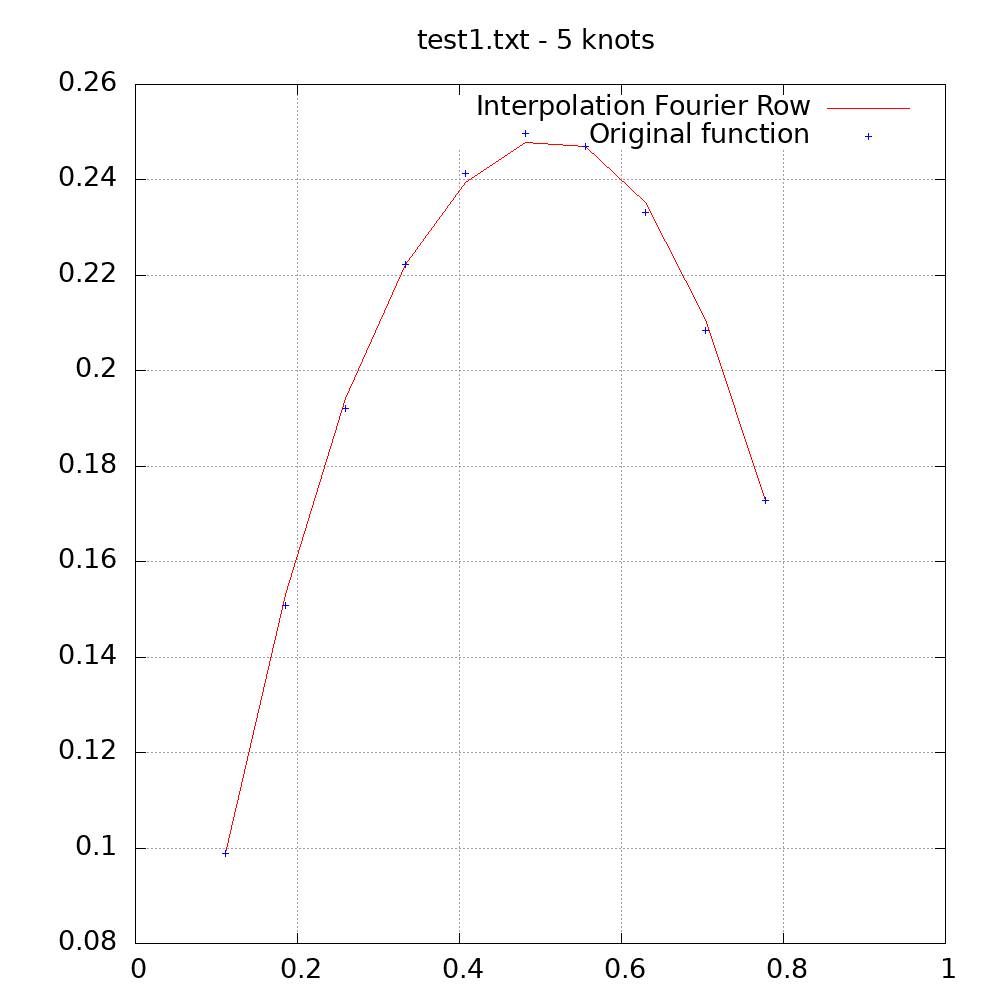
\includegraphics[scale=0.5]{Images/test1.txt.png}
        \caption{Результаты теста "Работоспособность".}
    \end{figure}
    \begin{figure}
        \centering
        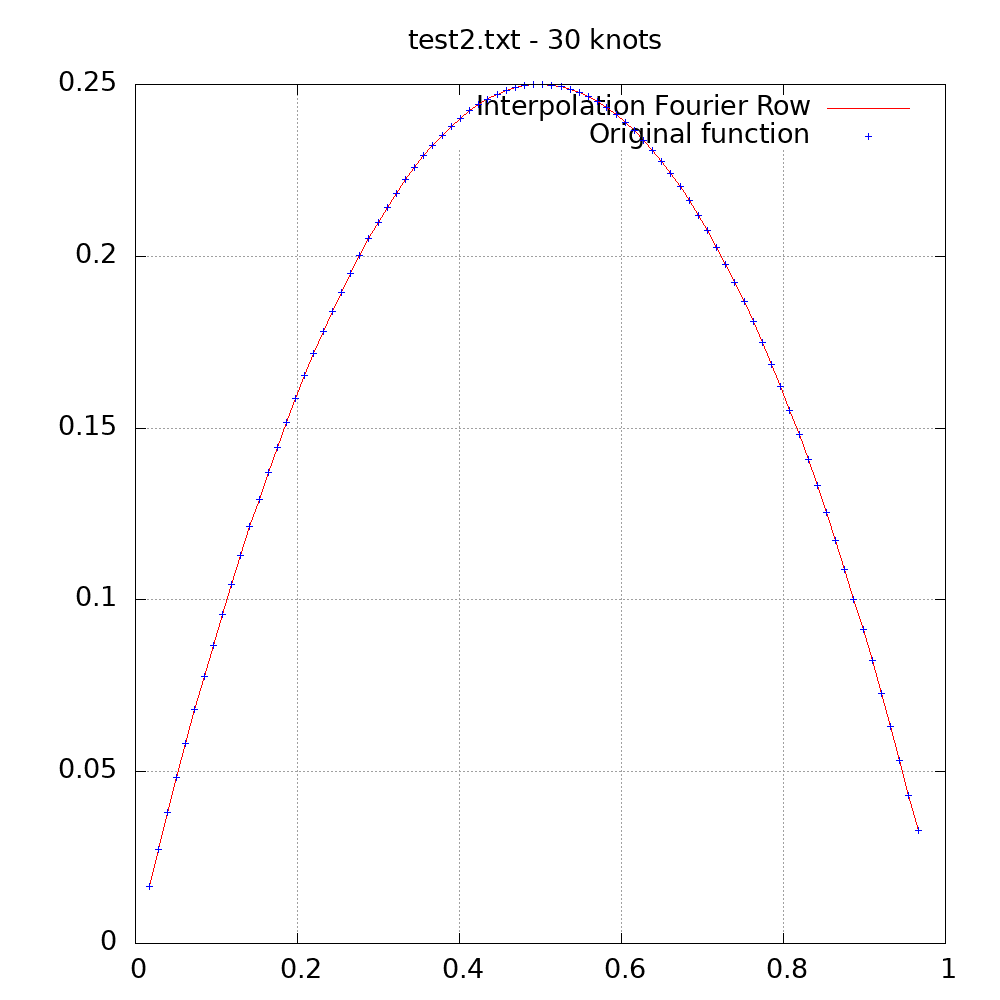
\includegraphics[scale=0.5]{Images/test2.txt.png}
        \caption{Результаты теста "Работоспособность".}
    \end{figure}
    \begin{figure}
        \centering
        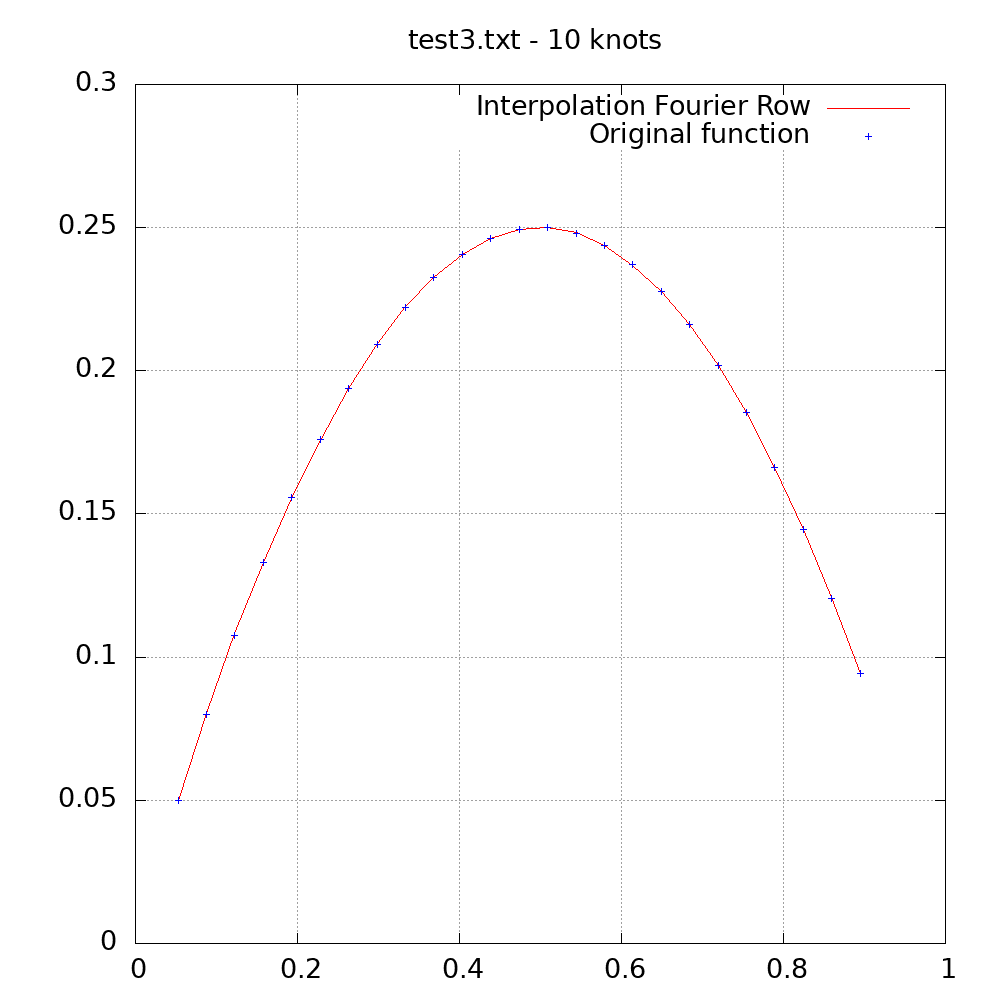
\includegraphics[scale=0.5]{Images/test3.txt.png}
        \caption{Результаты теста "Работоспособность".}
    \end{figure}
    \begin{figure}
        \centering
        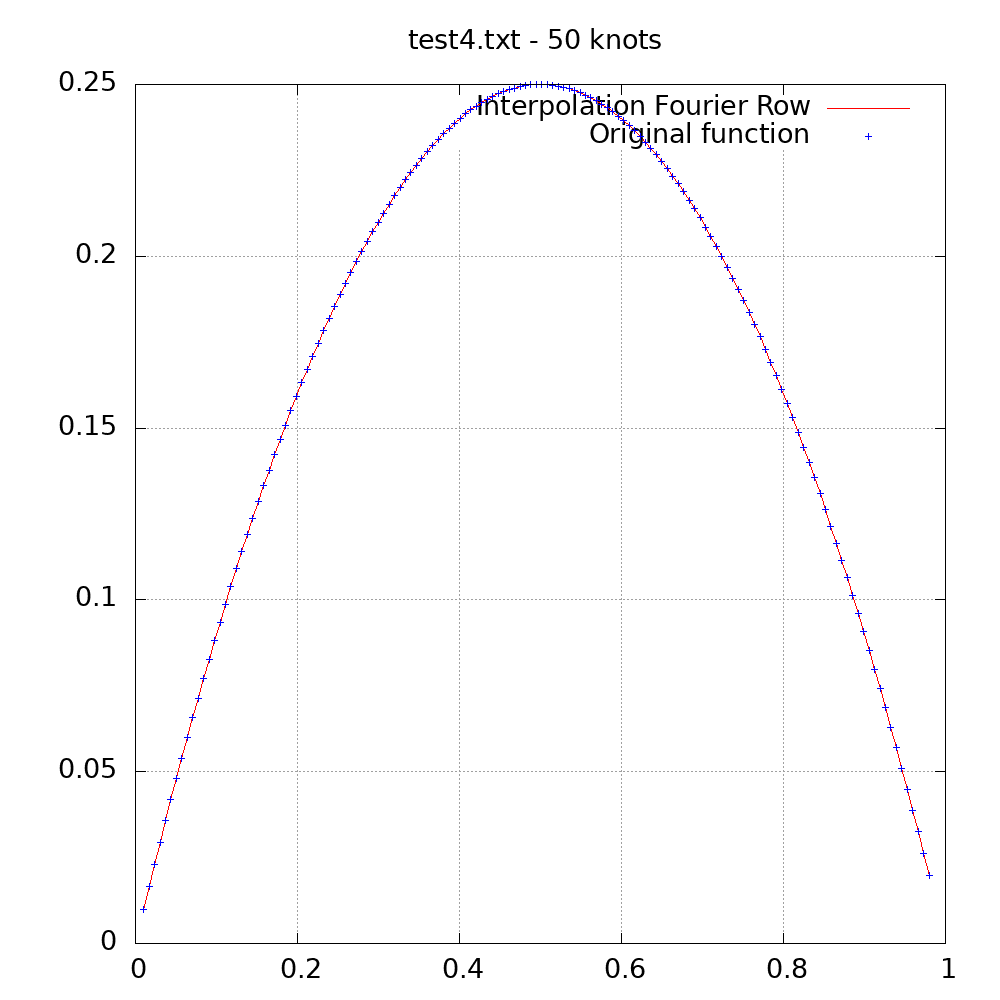
\includegraphics[scale=0.5]{Images/test4.txt.png}
        \caption{Результаты теста "Работоспособность".}
    \end{figure}

    \subsection{Численное нахождение $p$.}

    Рассматривалась та же функция. Вывод программы: 2.056901336970021.

    \begin{figure}
        \centering
        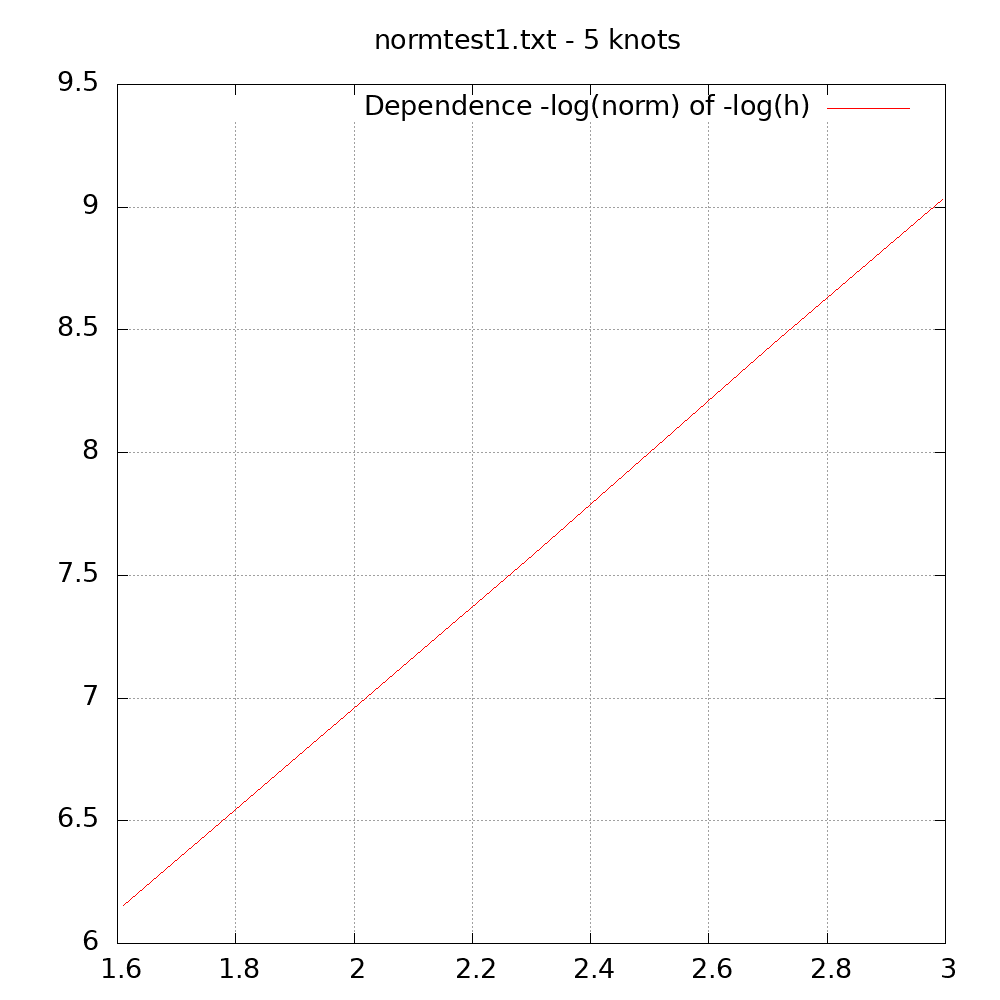
\includegraphics[scale=0.5]{Images/normtest1.txt.png}
        \caption{Результаты теста "Численное нахождение $p$".}
    \end{figure}

\end{document}